\documentclass{article}
\usepackage[utf8]{inputenc}
\usepackage[utf8]{ctex}
\usepackage{graphicx}

\title{应用于黑白棋的几种智能算法}
\author{16337341 朱志儒}
\date{January 2019}

\begin{document}


\maketitle

\section{摘要}
极具趣味性和挑战性的学科非人工智能莫属,许多科研人员都在为之奋斗,将人工智能算法应用于传统的棋类游戏是人们关注和研究人工智能的内容之一。黑白棋\cite{r3}是19世纪末英国人发明,上个世纪70年代日本人长谷川五郎将其发展的棋类游戏。
与其他棋类游戏(例如,中国象棋、国际象棋和围棋)相比,黑白棋每层搜索的节点数量并不是特别庞大,其游戏规则也较为简单,所以棋局的评估函数可以做的较为细致。
\par
本论文将设计并实现复杂的评估函数,并将强化学习中的Q-learning和Sarsa算法以及博弈树搜索中的Minimax算法和Alpha-beta剪枝算法这四种智能算法运用于黑白棋,比较这四种算法的智能程度以及效率。最后,经过测试,Alpha-Beta剪枝算法比Minimax算法在效率上有相当大的提高,且它们在黑白棋上的智能较高,而Sarsa与Q-learning则在黑白棋上的智能较低。

\section{引言}
黑白棋\cite{r3}使用{$8\times8$}的棋盘,下棋时将棋下在方格中间。开始时,在棋盘的正中间有两个黑棋和两个白棋交叉放置,黑棋先手,双发轮流落子。下子时必须在一个空位下子并且新落子的棋子必须与己方的棋子在同一直线(横、竖、斜)上夹着对方的棋子,这些被夹的棋子将转变成己方棋子。如果有一方没有合法位置下子,则对手可继续下子直到该方有位置可下。如果轮到一方下子且有位置可下,则其必须下子而不能弃权。黑白双方轮流下子,直到棋盘下满或双方都没有合法位置可下,则游戏结束,棋盘上棋子多的一方获胜。
\par
在黑白双方对弈的过程中,计算机需要对整个棋局进行分析和评估,将整个棋局为分多个方面的因素,每个因素根据重要性分配相应的权重,最后进行加权求和得到整个棋局的评估值。考虑的因素越多,对整个棋局的分析和评估也就越准确,但效率也就越底下。所以,对整个棋局的分析和评估需要考虑数量和效率,并做好二者的权衡。
\par
本论文在对棋局进行分析和评估时,将棋局抽象成下列因素:基于位置特征的估计值、基于黑白子比例的估计值、基于行动力的估计值、基于近角位的估计值、基于稳定子的估计值和基于角位的估计值,为这些因素分配不同的权重,最后将这些因素加权求和得到棋局的估计值。
\par
本论文的主要研究的内容是为黑白棋的棋局设计复杂的评估函数,将强化学习中的Q-learning算法和Sarsa算法以及博弈树搜索中的Minimax算法和Alpha-Beta剪枝算法运用到黑白棋,并比较这四种算法的智能程度以及效率。
\par


\section{方法}
\subsection{评估函数}
\subsubsection{基于位置特征的估计值}
黑白棋和围棋相似,有“金边银角草肚皮”的说法,棋子在四个角的优势巨大,因为在四角的棋子不可能被翻转;然而在近角位的优势小,因为这些位置容易让对方占角或是被对方翻转大量的棋子;四条边上的其他位置的优势也比较大,因为迅速占边可以比较容易地获得边界稳定子的优势;而在棋盘的中心位置优势较低。棋盘的所有位置的权重值如下:
\begin{center}
    \begin{tabular}{|c|c|c|c|c|c|c|c|}
        \hline 20&-3&11&8&8&11&-3&20 \\
        \hline -3&-7&-4&1&1&-4&-7&-3 \\
        \hline 11&-4&2&2&2&2&-4&11 \\
        \hline 8&1&2&-3&-3&2&1&8 \\
        \hline 8&1&2&-3&-3&2&1&8 \\
        \hline 11&-4&2&2&2&2&-4&11 \\
        \hline -3&-7&-4&1&1&-4&-7&-3 \\
        \hline 20&-3&11&8&8&11&-3&20 \\
        \hline
    \end{tabular}
\end{center}
\par
计算己方所有棋子权重的和与对方所有棋子权重的和,再相减就可以得到基于位置特征的估计值。

\subsubsection{基于黑白子比例的估计值}
在黑白棋中,如果己方棋子比对方棋子数量多,则说明己方占优,如果对方棋子比己方棋子数量多,则说明对方占优。在实际对战过程中,这项估计值的参考价值并不是特别大,因为黑白子比例与谁将下子关系很大,比如说,在己方棋子数目远小于对方棋子数目的情况下,己方着子后可能翻转对方大量的棋子,从而会逆转局势。所以黑白子比例的估计值在棋局估计值中占比较低。

\subsubsection{基于角位和近角位的估计值}
在黑白棋中,角位是无法被翻转的,占领角位将带来极大的优势,所以在角位附加一项极大的估计值。而落子于近角位将很可能把角位送给对方,这将会给己方带来极大的劣势,所以在近角位附加一项极小的负估计值。角位和近角位的估计值在棋局估计值占比较高。

\subsubsection{基于稳定子的估计值}
在黑白棋中,稳定子是棋局估计值的重要指标,拥有更多的稳定子,既能保证己方最少的棋子数,又能帮助己方翻转大量对方的棋子,形成成片稳定子的作用。稳定子可分为两种:内部稳定子和边界稳定子,内部稳定子的作用并没有比边界稳定子大,因为内部稳定子并不一定能帮助己方翻转对方棋子。计算内部稳定子的估计值时,只需为每个内部稳定子赋予一个相同的权重。对于边界稳定子的估计值的计算,从棋盘的一个角开始,权重分别为:
\begin{center}
    \begin{tabular}{|c|c|c|c|c|c|c|c|}
        \hline 1&2&3&4&5&6&7&8 \\
        \hline
    \end{tabular}
\end{center}
\par
这样设计权重将鼓励占边,形成成片的稳定子,加大优势。稳定子的估计值在棋局估计值中占比较大。

\subsubsection{基于行动力的估计值}
在黑白棋中,行动力是指棋盘上某一方的可下子位置个数,行动力较高时,可保证之后的若干步都会有较好的下法。与黑白子比例的估计值相似,行动力的估计值也采用比例算法,但需要考虑两种特殊情况:
\par
1. 如果己方没有位置下子,那么设置特低的行动力估计值
\par
2. 如果对方没有位置下子,那么设置特高的行动力估计值
\par
这样就可以避免己方处于无子可下的糟糕局面,而倾向于选择使对方无子可下的优势局面。行动力估计值在棋局估计值中占比较高。

\subsection{强化学习}
\subsubsection{Q-learning\cite{r1}}
Q-learning在黑白棋的应用中,每个不同的状态S表示每个不同的棋局,动作a表示下一步下子的位置,动作集A表示可下子位置的集合,状态S的即时回报R表示S所对应棋局的估计值。Q-learning在黑白棋中的步骤为:
\par
1. 初始化棋局S和表Q
\par
2. 进入循环,根据$\epsilon$-greedy算法在棋局$S_i$中选择下一步下子位置$A_i$,在位置$A_i$下子且对方也下完子后得到棋局$S_{i+1}$和$S_{i+1}$的估计值$R_{i+1}$,然后更新表Q,即
\begin{center}
    {Q($S_i$, $A_i$) = Q($S_i$, $A_i$) + $\alpha$($R_{i+1}$ + $\lambda$$max$Q($S_{i+1}$, $a_{i+1}$) - Q($S_i$, $A_i$))}
\end{center}
\par
其中$max$Q($S_{i+1}$, $a_{i+1}$)表示在棋局$S_{i+1}$中对于所有可下子位置选择对应最大的Q值。
\par
3. 不断循环直至游戏结束

\subsubsection{Sarsa\cite{r1}}
Sarsa在黑白棋的应用中,状态S、动作a、动作集A和即时回报R所表示的意义与Q-learning在黑白棋的应用相同,Sarsa在黑白棋中的步骤为:
\par
1. 初始化棋局S和表Q
\par
2. 进入循环,根据$\epsilon$-greedy算法在棋局$S_i$中选择下一步下子位置$A_i$,在位置$A_i$下子且对方也下完子后得到棋局$S_{i+1}$和$S_{i+1}$的估计值$R_{i+1}$,再根据$\epsilon$-greedy算法再棋局$S_{i+1}$中选择下一步下子位置$A_{i+1}$,然后更新表Q,即
\begin{center}
    {Q($S_i$, $A_i$) = Q($S_i$, $A_i$) + $\alpha$($R_{i+1}$ + $\lambda$Q($S_{i+1}$, $A_{i+1}$) - Q($S_i$, $A_i$))}
\end{center}
\par
3. 不断循环直至游戏结束

\subsection{博弈树搜索}
\subsubsection{Minimax算法\cite{r2}}
对博弈树进行深度优先搜索获得当前棋局之后的所有可能结果,玩家双方均会选择对自己最有利的走法,也就是说,对于己方而言,会选择最大化己方优势的走法,然而,对方会选择使己方优势最小化的走法。从博弈树来看,每一层轮流从子节点中选取MAX-MIN-MAX-MIN...
\begin{center}
    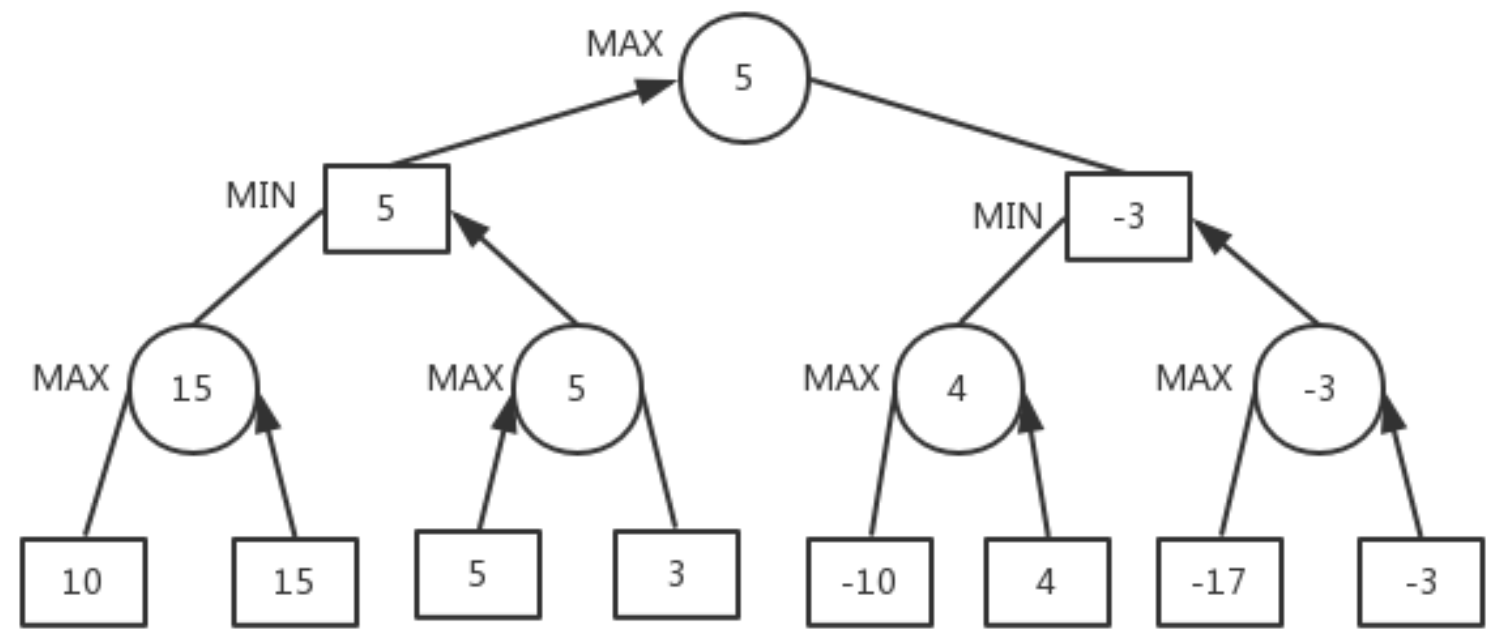
\includegraphics[scale=0.6]{1.PNG}
\end{center}
\par
深度优先搜索的深度限制为4层时,图中第4层为叶子节点;第3层为己方根据第4层的棋局估计值推出该层节点的棋局估计值,选取的是子节点中的最大值,即最大化自己的优势;第2层为对方根据第3层的棋局估计值推出该层节点的棋局估计值,选取的是子节点中的最小值,即最小化己方的优势;第1层为己方根据第2层棋局估计值推出该层节点的棋局估计值,选取的是子节点中的最大值,即最大化己方的优势,从而己方就可以得到下一步最大化优势的走法。

\subsubsection{Alpha-Beta剪枝算法\cite{r2}}
Alpha-Beta剪枝建立在Minimax算法的基础上,但它减少了Minimax算法搜索树的节点数。
\par
Alpha剪枝过程:对于MIN层的节点,如果估计出其倒推值的上确界beta小于或等于其MAX层父节点的估计倒推值的下确界alpha,即beta$\leq$alpha,则不必再扩展该MIN层的其余节点,因为其余节点的估计值如何已经不能改变父节点的MAX值了。
\par
Beta剪枝过程:对于MAX层的节点,如果估计出其倒推值的下确界alpha大于或等于其MIN层父节点的估计倒推值的上确界beta,即beta$\leq$alpha,则不必再扩展该MAX层的其余节点,因为其余节点的估计值如何已经不能改变父节点的MIN值了。
\begin{center}
    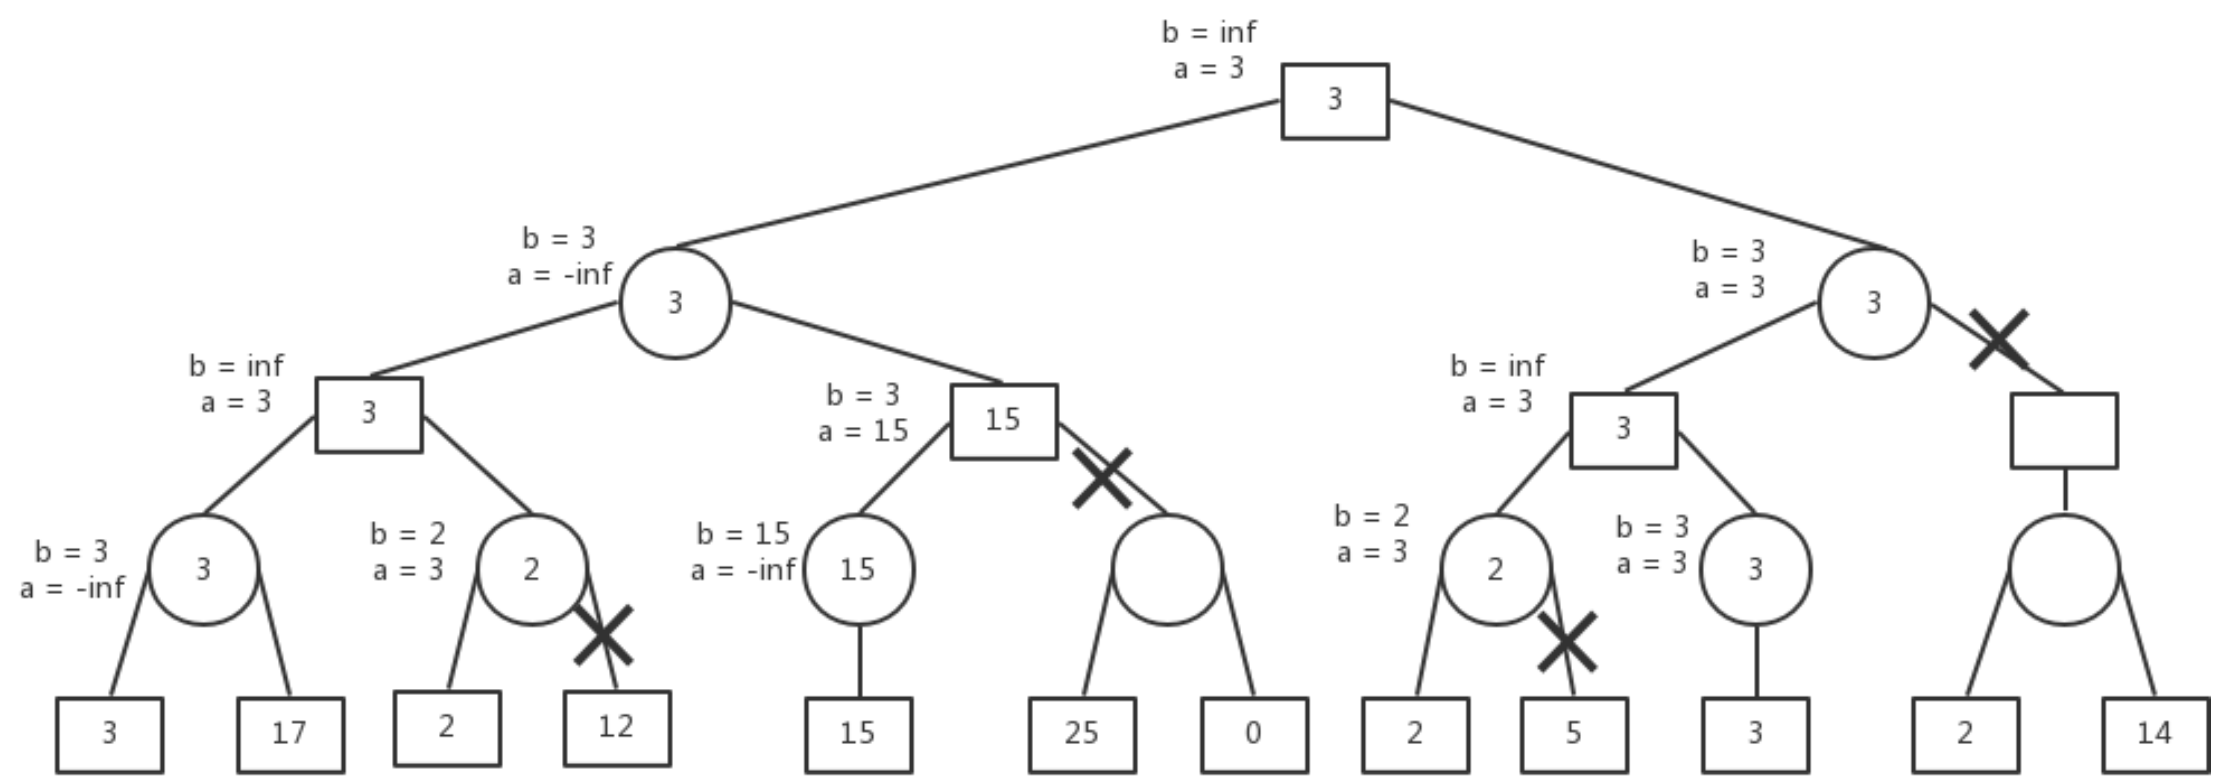
\includegraphics[scale=0.4]{2.PNG}
\end{center}
\par
如上图显示的Alpha-Beta剪枝过程,方框为MAX,圆圈为MIN。初始设置a = -$\infty$,b = +$\infty$,深度优先搜索到达左下角的节点,第四层MIN层取子节点中的最小值3,3 < b,则b = 3;回溯到第三层MAX层,3 > a,则a = 3,b不变还是为正无穷;深度优先搜索右子树到第五层,返回值为2;回溯到第四层MIN层节点,2 < b,则b = 2,而此时a = 3,就有b < a,所以进行剪枝,不用搜索第四层MIN节点的右子节点,第四层MIN层节点返回2;回溯到第三层MAX层节点,2 < 3,a不变,返回值为3;回溯到第二层MIN层节点,3 < b,则b = 3;深度优先搜索到第五层节点,返回值为15;回溯到第四层MIN层节点,没有其他的子节点,所以返回值为15;回溯到第三层MAX层节点,15 > a,则a = 15,此时b = 3,就有b < a,所以进行剪枝,不需要探索第三层MAX层节点的右子节点,第三层MAX层节点返回值为15;回溯到第二层MIN层节点,3 < 15,所以其返回值为3;回溯到根节点,3 > a,则a = 3,再深度优先搜索根节点的右子节点,同时剪枝,最后结果如上图。

\section{实验}
\subsection{强化学习}
将$\epsilon$设置为0.5,学习速率a设置为0.8,折扣因子$\lambda$设置为0.5,使用评估函数就可以得到每个棋局S的即时回报R。在训练Q-learning算法的模型时,与随机数对弈50万局;在训练Sarsa算法的模型时,与随机数对弈100万局。
\par
在实际对弈时,对于当前棋局S以及可下子位置集A,在训练后的表Q中寻找具有最大Q值的(S,a)对,可下子位置a就是当前棋局S最优的下子位置。如果训练后的表Q中没有与(S,A)对应的Q值,则随机选取A中的一个位置下子。
\par
训练好两个模型后分别与随机数进行博弈,对弈100局,下表为统计数据,train\_times表示训练时与随机数对弈的总局数,rate表示与随机数对弈100局的胜率,Q\_numbers表示训练train\_times局后表Q中存储的(S,A)对以及对应Q值的数量,avg\_hits表示在每局对弈中(S,A)对出现在训练后的表Q的频率。
\begin{center}
    \begin{tabular}{ccccc}
        \hline
         & train\_times & rate & Q\_numbers & avg\_hits \\
        \hline
        Q-learning & 500000 & 68\% & 12559838 & 27\% \\
        Sarsa & 1000000 & 69\% & 24834550 & 43\% \\
        \hline
    \end{tabular}
\end{center}

\subsection{博弈树搜索}
在实际对弈中,以当前棋局作为根节点,进行深度优先搜索,搜索深度限制为6,在搜索的同时,以Minimax算法或Alpha-Beta剪枝算法构建博弈树,博弈树中叶子节点的估计值由评估函数得到,搜索并构建好整个博弈树后就可以得到最优的下子位置。
\par
本论文选择与随机数进行博弈,对弈100局,下表为统计数据,其中depth表示搜索深度,rate表示与随机数对弈100局的胜率,nodes表示搜索过的节点总数。
\begin{center}
    \begin{tabular}{cccc}
        \hline
         & depth & rate & nodes \\
        \hline
        Minimax & 6 & 92\% & 5328243 \\
        Alpha-Beta & 6 & 92\% & 2939082 \\
        \hline
    \end{tabular}
\end{center}

\section{结论}
从实验中可以看出,强化学习中的Q-learning和Sarsa并不适合黑白棋,因为黑白棋具有太多的棋局和对应每个棋局不同的下子位置,这导致实际运用中根本无法存储这么多种情况。在统计数据中,每次与随机数对弈时在表Q中找到对应的(S,A)的频率也只有27\%和43\%。再者它与随机数对弈训练,这导致每次训练的棋局也会有所不同,从而Q表中对应的值收敛较慢,即使训练100万次,但对于1亿多个棋局和下子位置,这些训练次数无法使得它们对应的Q值收敛,对弈时并不能找到最优的下子位置,所以可以得出,Sarsa算法与Q-learning算法还存在一定的局限性,因为它们的胜率远小于博弈树搜索算法的胜率。
\par
因此,Minimax算法以及进行Alpha-Beta剪枝优化以提升计算速度是更适合黑白棋的,从实验结果展示可以看出它们的胜率远远高于另外两个。且在相同的搜索深度条件下,Alpha-Beta剪枝探索的节点数远远小于Minimax算法探索的节点数。

\begin{thebibliography}{10}
\bibitem{r1} Sutton R S, Barto A G. Reinforcement learning: An introduction[J]. 2011.
\bibitem{r2} 王永庆. 人工智能原理与方法[M]. 西安: 西安交通大学出版社,
1998: 288-290.
\bibitem{r3} 黑白棋. 百度百科. (2018-9-16) https://baike.baidu.com/item/%E9%BB%91%E7%99%BD%E6%A3%8B/80689
\end{thebibliography}

\end{document}